\section{Approach}\label{sec:approach}

\subsection{Simulation}

%END SIM - MERGE ANCHOR
\subsection{Boot Protection}
The C\&DH system uses a Linux kernel that is booted by
U-boot.\footnote{\url{http://www.denx.de/wiki/U-Boot}} The fault model
considered here is bit corruption in the Linux kernel that is present at boot
time.  Currently, there is only one copy of the Linux kernel and if it fails to
boot, the entire C\&DH system will experience catastrophic failure.  The
solution described below is designed to reduce that single point of failure to a
much smaller region of code.

\subsubsection{Test Environment}
In order to develop and test the boot protection system in a controlled
environment, we decided to use an ARM emulator.  The QEMU~\cite{bellard2005qemu}
emulator is well known and supports a variety of architectures, including
several ARM development boards.  It does not currently support the MityARM board
used by IlliniSat, so we use the ``versatilepb'' virtual development board to
run U-boot and Linux compiled for
ARM.\footnote{\url{http://elinux.org/Virtual_Development_Board}}

The initial bulk of this work involved getting the test environment running and
we have made detailed notes so that we can share this procedure with others
working on similar problems.  The versatilepb board in QEMU has a virtual flash
drive that is memory mapped to address 0x3400000, which we use to store the
contents of the OS kernel images and the boot protection scheme.

U-Boot has built-in support for CRC-32, and every image (e.g. application, OS,
script, filesystem, etc...) is stored in a format that contains this checksum.
Therefore, one can use this built-in functionality to validate checksums.  


%(1.7 megabytes) / (914 bytes) = 1950.30547

%Include: SD card and memory map stuff
\begin{figure}
  \centering
  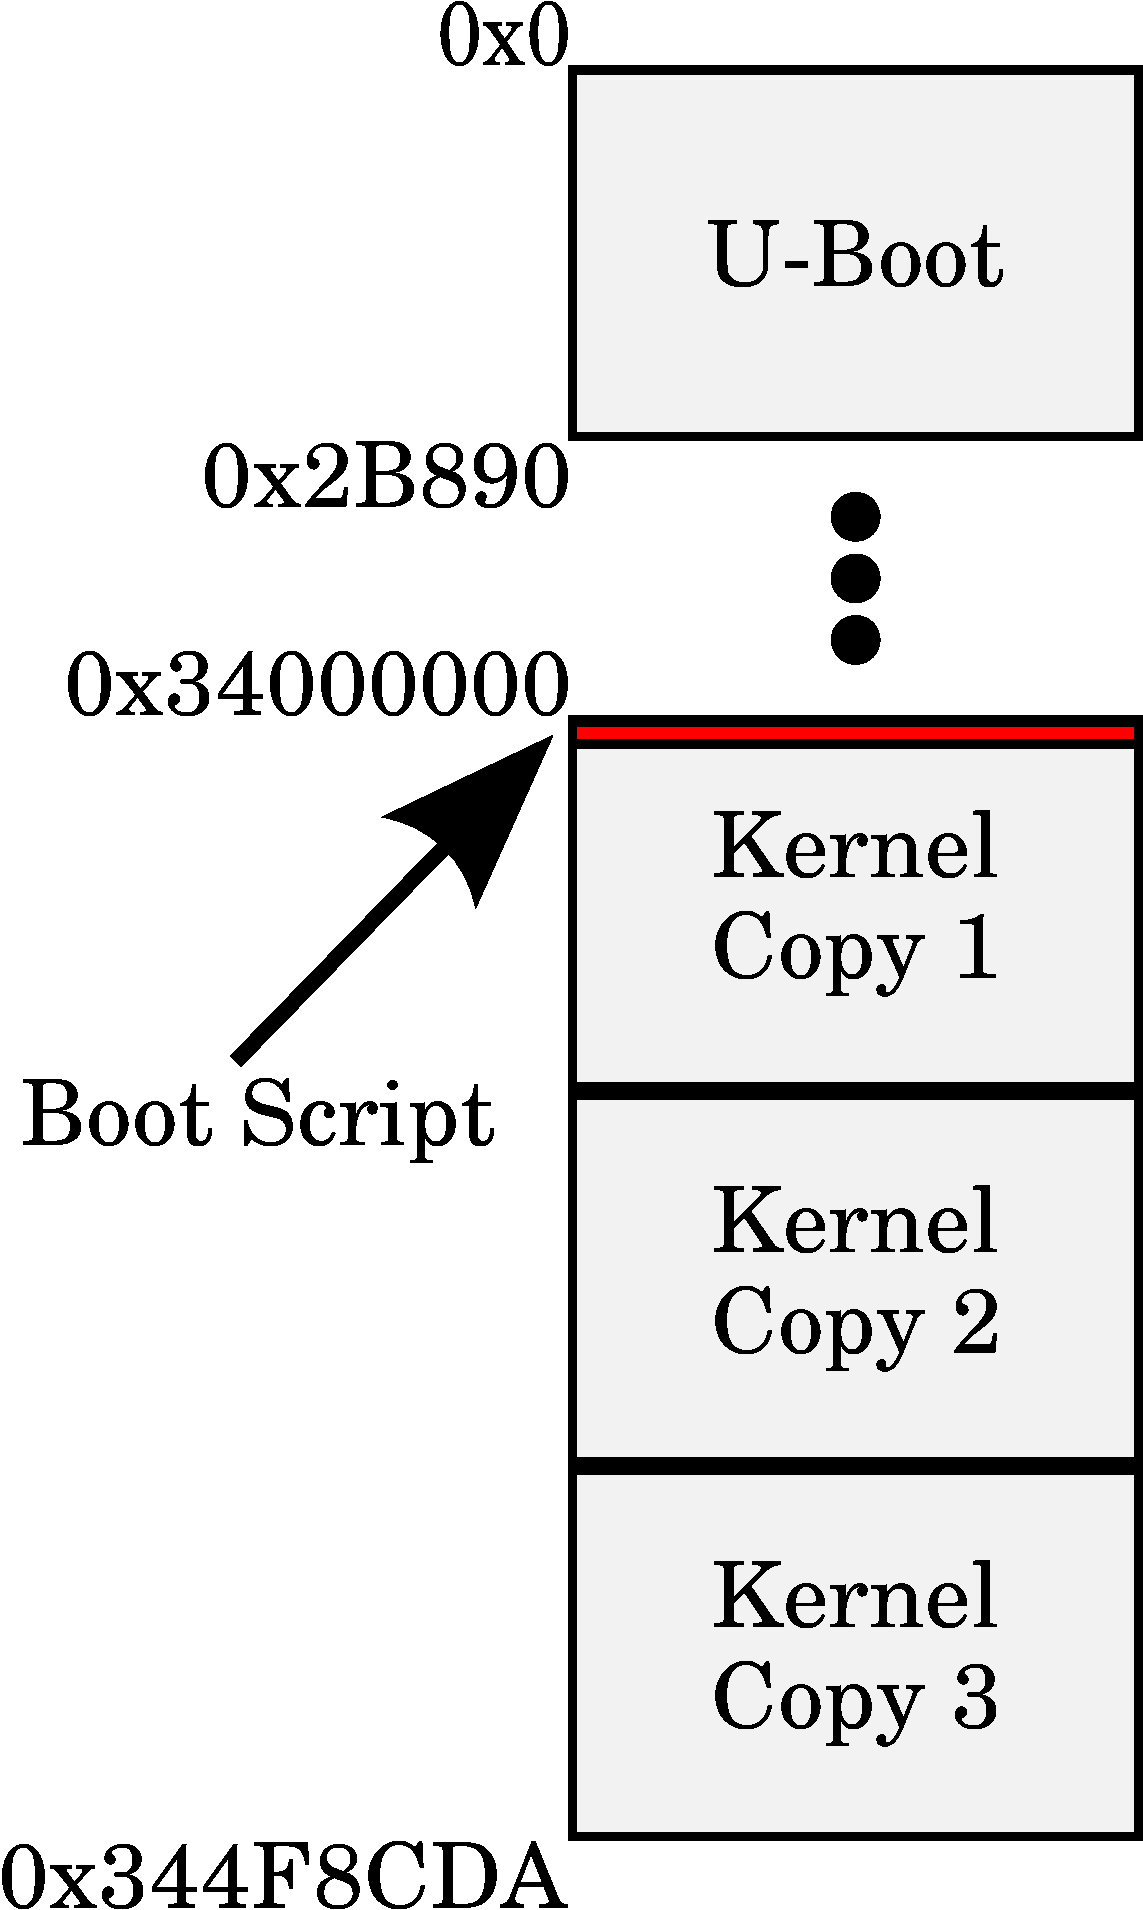
\includegraphics[width=0.15\textwidth]{images/mem_map}
  \caption{The memory map used to evaluate the boot protection system in QEMU.
           The U-boot application itself occupies 0.17MB, whereas the protection
           script is 914 bytes and each Linux kernel is
           1.7MB.}\label{fig:mem_map}
\end{figure}

%END BOOT - MERGE ANCHOR
\subsection{Flash Patrol Read Daemon}
